% Figure source: representation-level perturbation response for BIBM 2026.
% Values are balanced accuracy from the manuscript tables.
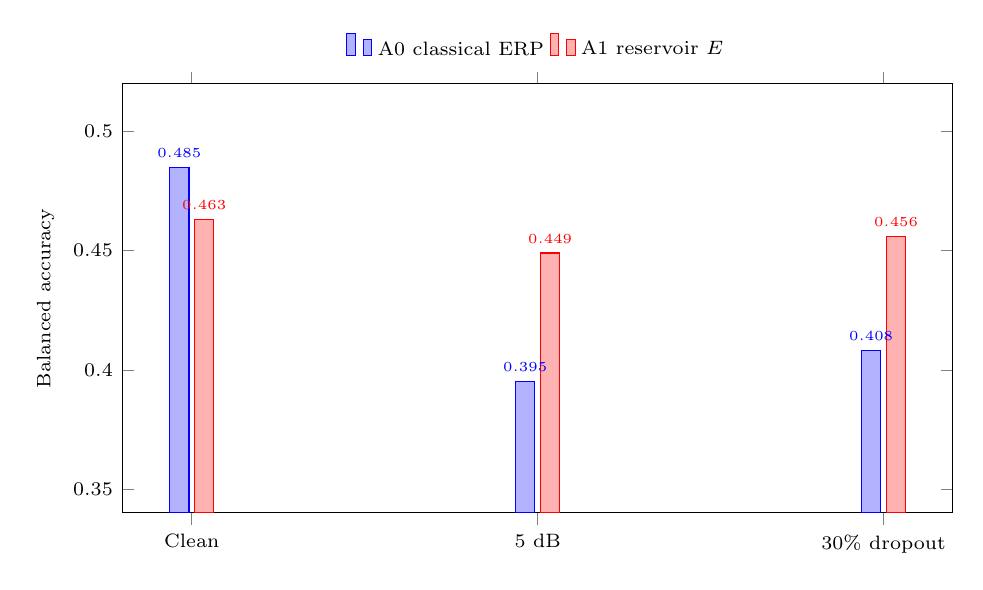
\begin{tikzpicture}
\begin{axis}[
    width=\linewidth,
    height=0.58\linewidth,
    ybar,
    bar width=7pt,
    ymin=0.34,
    ymax=0.52,
    ylabel={Balanced accuracy},
    symbolic x coords={Clean,5 dB,30\% dropout},
    xtick=data,
    x tick label style={font=\scriptsize, align=center},
    y tick label style={font=\scriptsize},
    label style={font=\scriptsize},
    legend style={font=\scriptsize, at={(0.5,1.03)}, anchor=south, legend columns=2, draw=none},
    nodes near coords,
    nodes near coords style={font=\tiny, /pgf/number format/fixed, /pgf/number format/precision=3},
    every axis plot/.append style={draw=black}
]
\addplot coordinates {(Clean,0.485) (5 dB,0.395) (30\% dropout,0.408)};
\addplot coordinates {(Clean,0.463) (5 dB,0.449) (30\% dropout,0.456)};
\legend{A0 classical ERP, A1 reservoir $E$}
\end{axis}
\end{tikzpicture}
